\section{Implementación}

En este apartado explicaremos la implementación que se ha llevado a cabo del juego Pacman, haciendo hincapié por una parte en los apartados gráfico y lógico del juego, y por otra centrándonos en cada uno de los apartados en los que se ha aplicado generación procedimental y el método desarrollado para cada caso.

\subsection{Implementación del juego base}

\subsubsection{Apartado gráfico}

Aunque se haya usado una biblioteca gráfica que nos permite cargar modelos \acrshort{3d}, se ha optado por la creación de los modelos tanto de Pac-Man como de los fantasmas a partir de formas geométricas simples. A su vez, se ha usado materiales simples y basados en los del juego original y un fondo negro como en el mismo.\\

Inicialmente, se siguió la misma estética minimalista para la representación gráfica del laberinto y sus componentes, optando por cubos azules y verdes con un borde blanco para los muros y los \textit{`pasillos''} o \textit{`portales''}, y por esferas blancas pequeñas y grandes para los puntos y las \textit{`pastillas''}. Posteriormente, se ha trabajado en la generación procedimental de texturas para los muros del laberinto y en un modelo \acrshort{3d} simple compuesto por un toro y una esfera para los portales.\\

\begin{figure}[H]
    \begin{center}
        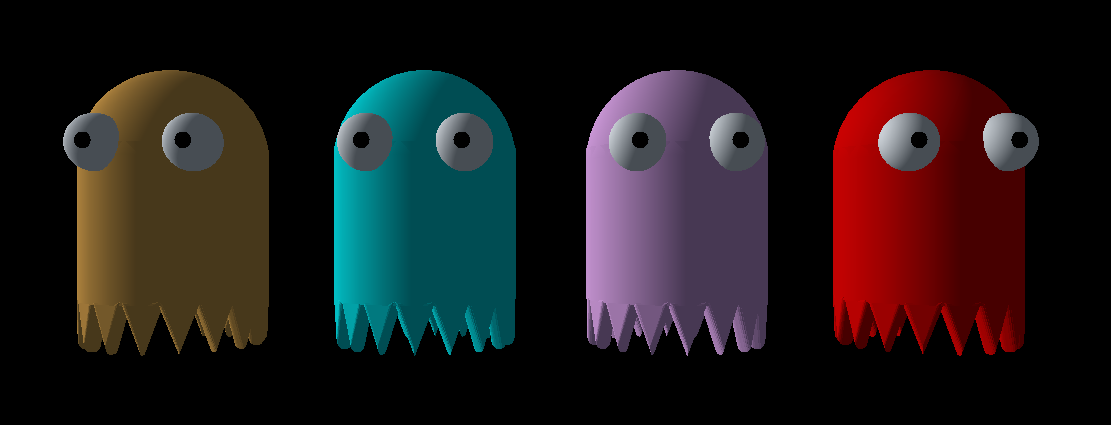
\includegraphics[scale=0.3]{img/fantasmas.png}
        \caption{Modelo \acrshort{3d} de los fantasmas.}
    \end{center}
\end{figure}

En lo que se refiere a las luces, se ha optado por una luz ambiente para evitar se vean negras aquellas zonas donde no incida otra fuente de luz y por una luz focal blanca situada en la parte superior izquierda del escenario.\\

En cuanto a la visualización, se ha creado una cámara en perspectiva, ya que utiliza la proyección en perspectiva que imita al ojo humano, método más utilizado en el renderizado de escenas \acrshort{3d}.

\newpage

\subsubsection{Apartado lógico}

\paragraph{Inteligencia artificial}

Más allá de los factores que modifiquen procedimentalmente el comportamiento de los fantasmas, se ha optado por un algoritmo de búsqueda de caminos \acrshort{astar} básico que utiliza la distancia Manhattan como medida heurística, ya que a efectos prácticos, las distancias que estamos midiendo son las de una cuadrícula y los personajes no cuentan con movimientos en diagonal, teniendo solo que preocuparnos de desplazamientos horizontales y verticales.\\

Por otra parte, los fantasmas cuentan con una máquina de estados que define su comportamiento, definiendo su casilla objetivo en función del estado en el que se encuentren tal y como hacía el juego original.\\

Los estados con los que cuentan son: permanecer en casa, perseguir a Pac-Man, huir de Pac-Man, volver a casa y quedarse quietos. Entre la figura \ref{fig:estados} y la tabla \ref{tab:estados} podemos observar la máquina de estados compuesta por estos cinco estados y las condiciones que deben cumplirse para saltar de un estado a otro.\\

 \begin{figure}[H]
        \begin{center}
            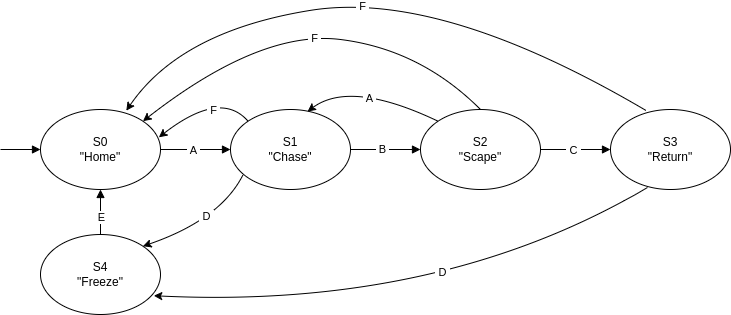
\includegraphics[scale=0.6]{img/estado_fantasmas.png}
            \caption{Máquina de estados que define el comportamiento de los fantasmas.}
            \label{fig:estados}
        \end{center}
    \end{figure}    
    
Aunque en los estados principales de perseguir a Pac-Man e huir de él son similares al juego original, la máquina de estados implementada nos ha permitido controlar en todo momento el comportamiento deseado de los fantasmas, ya que por ejemplo, cuando un fantasma está volviendo a casa solo queremos que se vea afectado por eventos ``radicales'' como que el jugador muera o el jugador supere el nivel actual.

\begin{table}[H]
\centering
    \caption{Condiciones y eventos que provocan un cambio de estado en los fantasmas.}
    \begin{tabular}{|c|l|c|}
    \hline
Variable & Condición                                                                                  & Transición                                                                                        \\ \hline
A        & Ha pasado un tiempo variable                                                               & \begin{tabular}[c]{@{}l@{}}$S0\rightarrow S1$\\ $S2\rightarrow S1$\end{tabular}                     \\\hline
B        & \begin{tabular}[c]{@{}l@{}}Pac-Man se ha comido una\\ píldora de energía\end{tabular}      & $S1\rightarrow S2$                                                                                 \\\hline
C        & \begin{tabular}[c]{@{}l@{}}Pac-Man se ha comido a\\ ese fantasma\end{tabular}              & $S2\rightarrow S3$                                                                                 \\\hline
D        & \begin{tabular}[c]{@{}l@{}}Un fantasma ha atrapado\\ a Pac-Man\end{tabular}                & \begin{tabular}[c]{@{}l@{}}$S1\rightarrow S4$\\ $S3\rightarrow S4$\end{tabular}                     \\\hline
E        & \begin{tabular}[c]{@{}l@{}}Ha terminado la animación \\ de muerte del Pac-Man\end{tabular} & $S4\rightarrow S0$                                                                                 \\\hline
F        & \begin{tabular}[c]{@{}l@{}}Se produce un cambio de\\ nivel\end{tabular}                    & \begin{tabular}[c]{@{}l@{}}$S1\rightarrow S0$\\ $S2\rightarrow S0$\\ $S3\rightarrow S0$\end{tabular} \\\hline
\end{tabular}
\label{tab:estados}
\end{table}

\paragraph{Controles, movimiento y colisiones}

En lo referido al movimiento de los fantasmas y al movimiento y controles de Pac-Man se ha implementado un movimiento lineal, avanzando siempre hacia la dirección hacia la que mira el modelo. Además, esto va acompañado de la posibilidad de girar en las cuatro direcciones para Pac-Man en todo momento y en tres de ellas para los fantasmas, ya que no se les permite realizar giros de 180 grados.\\

En cuanto a las colisiones, se gestionan utilizando cajas de colisión o \textit{hitboxes}. Es un sistema sencillo que nos permite interaccionar tanto con los objetos de nuestro entorno como los muros, los portales o los potenciadores como con los fantasmas.\\

Por último, de cara a mejorar la jugabilidad y manejabilidad del personaje, se han implementado dos mecánicas de movimiento para Pac-Man. En primer lugar, los giros se realizan mediante un buffer que recuerda la última dirección indicada por el jugador y realiza el giro cuando llega a una intersección en la que el movimiento almacenado está permitido. Además este buffer se va actualizando siempre a la última instrucción dada, por lo que facilita la navegabilidad del laberinto. En segundo lugar, se ha implementado un giro ``tardío'' o más permisivo, es decir, que se nos permitirá girar en una intersección incluso si el personaje ha comenzado ya a salir de la misma.\\

Todo esto genera un sistema y unos controles sencillos y permisivos a la vez que precisos, mejorando la experiencia de usuario.

% ---------------------------------------------------------------------------- %

\newpage

\subsection{Generación de laberintos}

En la implementación se han representado los laberintos como una matriz \textit{mazeData}, conteniendo cada una de sus celdas un entero entre 0 y 4 que se traduce en un elemento \textit{MyTile}, formando el mapa final. En el proyecto se han implementado dos métodos, la generación tradicional manual y el grueso de este proyecto, una implementación utilizando generación procedimental.

\begin{table}[H]
    \centering
    \caption{Tipos de baldosas que componen los laberintos.}
    \begin{tabular}{|c|c|c|}
    \hline
    Valor   & Significado & Representación        \\ \hline
    {[}0{]} & Muro        & Cubo azul             \\ \hline
    {[}1{]} & Camino      & Cubo transparente     \\ \hline
    {[}2{]} & Punto       & Esfera blanca pequeña \\ \hline
    {[}3{]} & Pastilla    & Esfera blanca grande  \\ \hline
    {[}4{]} & Portal      & Modelo propio            \\ \hline
    \end{tabular}
\end{table}

\subsubsection{Generación manual}

Es el método estándar basado en laberintos pre-establecidos, no siendo más que la mera representación de nuestro mapeado en la matriz ya citada, introduciendo los datos previamente en nuestro programa. Los laberintos generados manualmente son de tamaño 31x28, tamaño de los mapas originales de Pac-Man. Sin embargo, debido a la sencillez del método, se pueden generar laberintos con otras dimensiones. Aunque sea tan simple, se ha querido hacer mención al mismo ya que ha sido fundamental de cara al desarrollo de la aplicación, permitiendo generar mapas concretos de cara a la realización de pruebas.

\subsubsection{Usando PCG}

El método que se ha desarrollado es una variación basada en la propuesta y explicación de Shaun LeBron \cite{lebron2012}, partiendo de la utilización de piezas de estilo Tetris como propone Lebron pero desarrollando un algoritmo propio para la generación procedimental y aleatoria de laberintos estilo Pac-Man de tamaño 30x30.\\

El método propuesto e implementado se divide principalmente en tres pasos:

\begin{enumerate}
    \item Generación de un modelo simple estilo Tetris.
    \item Conversión a un modelo de caminos.
    \item Creación de otros elementos y modelado final.
\end{enumerate}

En las siguientes secciones describiremos el proceso de generación procedimental de los laberinto y el funcionamiento del algoritmo propio diseñado para tal propósito. Además, en la sección \ref{par:ejemplo} se explicará el proceso mediante imágenes para un caso reducido.

\paragraph{Modelo simple}
Nuestro objetivo es crear una matriz de tamaño 9x5 que rellenaremos de piezas estilo Tetris. Antes de entrar en los detalles del método implementado, debemos definir la representación de las celdas de nuestra matriz y de las consideraciones previas que debemos tener en cuenta para cumplir con los patrones de diseño de niveles establecidos el juego Pac-Man.\\

Como representación de cada celda hemos escogido una tupla de dos elementos que representan si dicha celda tiene borde en su parte superior y en su lateral derecho. Esta representación nos deja cuatro tipos de celdas, la que tiene ambos bordes, la que no tiene ninguno, la que tiene solo el de la derecha y la que tiene solo el de arriba.\\

\begin{figure}[H]
    \begin{center}
        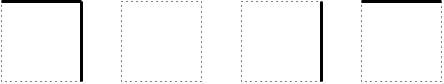
\includegraphics[scale=0.55]{img/celdas.png}
        \caption{Representación de los cuatro tipos de celdas.}
    \end{center}
\end{figure}

Gracias a esta definición, podemos crear un tablero completo de una manera eficiente, ya que los bordes que no definimos en una celda los definen las celdas colindantes. Si guardásemos las cuatro posiciones (arriba, abajo, derecha e izquierda) duplicaríamos la información de los bordes compartidos entre dos piezas.\\

Sin embargo, esta representación no nos permite representar a priori los bordes situados en el lateral izquierdo de las piezas de la primera columna ni los bordes inferiores de las piezas de la última fila, tal y como podemos ver en la figura \ref{fig:representacionColor}.\\

Ambos problemas los solucionaremos más adelante, por lo que por ahora los dejaremos apartados temporalmente. Por otra parte, en la generación de esta matriz 9x5 debemos tener en cuenta que tantos los fantasmas como Pac-Man tienen la misma posición de inicio independientemente del mapa generado, por lo que debemos asegurar que dichas posiciones queden disponibles para los personajes.\\

Por ello aseguraremos, independientemente de la disposición aleatoria de las piezas estilo Tetris, que nuestro modelo simple contendrá las celdas que componen la \textit{``casa''} de los fantasmas (representada por el cuadrado amarillo en la figura \ref{fig:representacionColor}) y que existe un borde en la primera columna, entre la séptima y octava filas, ya que será el punto de aparición de Pac-Man.\\

\begin{figure}[H]
    \centering
        \begin{subfigure}[b]{0.45\textwidth}
            \centering
            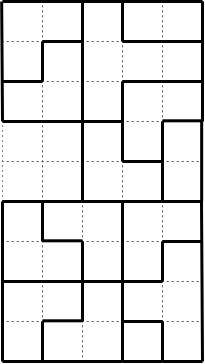
\includegraphics[scale=0.65]{img/grafo.png}
            \caption{Representación simple de los bordes de las piezas.}
        \end{subfigure}
        \hfill
        \begin{subfigure}[b]{0.45\textwidth}
            \centering
            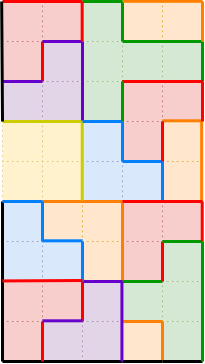
\includegraphics[scale=0.65]{img/grafo_color.png}
            \caption{Representación de los bordes coloreados por piezas.}
        \end{subfigure}
        \caption{Comparación entre los bordes a definir y los definidos utilizando celdas.}
        \label{fig:representacionColor}
\end{figure}


Tomadas estas consideraciones previas, podemos entrar en detalle en qué piezas estilo Tetris usaremos y cómo las añadiremos a nuestra matriz para obtener finalmente el modelo simple. En cuanto a las piezas, definiremos cada pieza como un conjunto de tres-tuplas con N elementos, siendo N el número de cuadrados que compongan la pieza, tuplas que corresponderán a la posición relativa\footnote{El eje Y está invertido debido a que utilizaremos estos valores para recorrer la matriz a la hora de comprobar si la posición de la pieza es válida.} de cada una de las celdas dentro de la pieza (fila, columna) y al tipo de celda que corresponde.\\

\begin{figure}[H]
    \begin{center}
        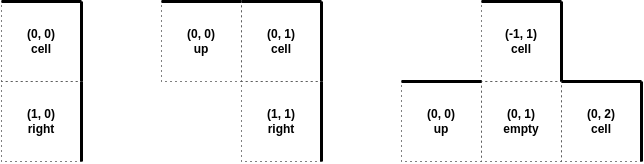
\includegraphics[scale=0.6]{img/piezas.png}
        \caption{Ejemplos de representación de varios tipos de piezas.}
    \end{center}
\end{figure}

A la hora de rellenar nuestra matriz con las piezas, la recorreremos por columnas y seguiremos el siguiente algoritmo de generación por procedimientos:

\begin{enumerate}
    \item Seleccionamos una casilla aleatoria de la columna actual de entre las que no han sido asignadas todavía a una pieza.
    \item Creamos un conjunto de piezas válidas.
    \begin{enumerate}
        \item Seleccionamos una pieza.
        \item Recorremos sus celdas comprobando que su posición relativa respecto a la casilla inicial que seleccionamos se encuentra sin asignar en nuestra matriz.
        \item Repetimos hasta quedarnos sin piezas.
    \end{enumerate}
    \item Seleccionamos una pieza aleatoria del conjunto de piezas válidas\footnote{En el caso de que nos encontrásemos con el conjunto vacío, asignaríamos por defecto una pieza con una única celda con borde en ambos lados.}.
    \item Asignamos los valores de las celdas de la pieza seleccionada a las respectivas posiciones de la matriz.
    \item Repetimos hasta completar la matriz.
\end{enumerate}

Debido a las transformaciones que sufrirá nuestra matriz en la creación del modelo de caminos, en la primera columna hemos definido un conjunto de piezas menor que en el resto. Esta consideración se ha tenido también en la última columna, pero esta vez con el fin de ahorrar comprobaciones innecesarias.\\

Finalmente, antes de pasar al siguiente modelo, solucionaremos el problema de los bordes de la última fila añadiendo una fila a nuestra matriz 9x5 que contenga celdas con únicamente borde superior.

\newpage

\paragraph{Modelo de caminos}

Con el modelo simple creado ahora contamos con una matriz 10x5 que representa los bordes que forman nuestras piezas estilo Tetris.\\

Si observamos nuestro modelo simple, podemos llegar fácilmente a la conclusión que los bordes representados en él no son más que los caminos que formaran nuestro laberinto y que los espacios restantes serán los muros del mismo. Además, también podemos observar que los caminos generados no crean ningún \textit{``callejón sin salida''}, ya que cada nodo del grafo generado cuenta con al menos dos caminos conectados.\\

Ya que nuestro objetivo es crear un laberinto de proporciones similares al laberinto original de Pac-Man de 31x28, si transformamos cada celda de nuestro modelo simple en una nueva de tamaño 3x3, obtendremos una matriz de 30x15. Cada una de nuestras celdas se traducirá convirtiendo los bordes en caminos y los espacios en blanco en muros, tal y como indica la siguiente figura.\\

\begin{figure}[H]
    \begin{center}
        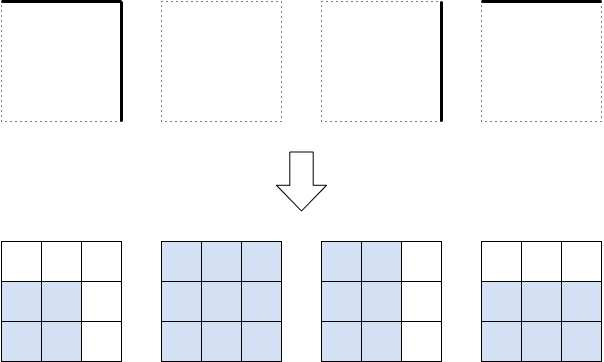
\includegraphics[scale=0.4]{img/celdas3x3.png}
        \caption{Transformación de celdas simples a casillas 3x3.}
    \end{center}
\end{figure}

Aunque las transformaciones propuestas del modelo simple al modelo de caminos implican una traducción casi perfecta de bordes a caminos, se genera una excepción muy específica en la que el modelo no se comporta como debería.\\

Este caso se da cuando encontramos una celda sin bordes con una celda con al menos un borde superior a su derecha y una celda con al menos un borde derecho encima suya. Sin embargo, este caso es fácilmente seleccionable, ya que cuando se de simplemente tendremos que sustituir el valor de la esquina superior derecha de nuestra casilla 3x3 por el de un camino.

\begin{figure}[H]
    \begin{center}
        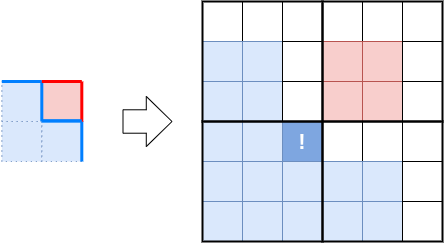
\includegraphics[scale=0.5]{img/grafo3x3.png}
        \caption{Excepción generada por las transformaciones propuestas.}
    \end{center}
\end{figure}

Con esta excepción ya contemplada y con el fin de cumplir con la simetría presente en los laberintos originales del juego, el siguiente paso que debemos dar es el de generar una matriz 30x30 en la que una mitad sea la inversa respecto al eje Y que la otra.\\

Sin embargo, debido a los modelos propuestos y transformaciones realizadas, debemos realizar dos últimos ajustes a nuestro modelo de caminos antes de dar este paso, ya que si se observa detalladamente, el modelo está rodeado de caminos\footnote{Con la excepción del borde inferior, que por el ajuste que hicimos en el modelo simple, ya cuenta con un muro exterior.} mientras que los laberintos deben estar rodeados por muros exteriores.\\

Por ello, actualmente nos faltaría un muro exterior en la primera fila y uno en el lado derecho de nuestro modelo. El primer caso se soluciona con un simple cambio, ya que contamos con dos filas de muro exterior en la parte inferior, desplazando todas las filas una posición hacia abajo y sustituyendo la primera por una de muro.\\

En el segundo caso aprovecharemos para retomar el problema que dejamos pendiente en el modelo simple. Como en el modelo simple no representamos correctamente los bordes de la izquierda de la primera columna, simplemente eliminaremos esa primera columna de nuestro modelo de caminos, dejando espacio para una columna de muro exterior en el extremo derecho de nuestra matriz.\\

Finalmente ya podemos realizar la simetría respecto al eje Y hacia la izquierda, obteniendo una matriz de 30x30 compuesta por caminos y muros.

\newpage
\paragraph{Modelo final}

Con el modelo de caminos terminado, contamos con un laberinto de tamaño 30x30 compuesto de muros y caminos. Por lo tanto, únicamente nos queda dotar a nuestra matriz de los elementos restantes del juego.

\begin{enumerate}
    \item Generación de portales.
    \item Generación de puntos.
    \item Generación de pastillas.
\end{enumerate}

Con el fin de generar más variedad aún de laberintos, se han añadido variantes \textit{``sin camino''} al conjunto de piezas de la última columna, generando posibles \textit{``callejones sin salida''}. Sin embargo, de cara a la generación de portales, supone una gran ventaja, ya que se generan automáticamente posiciones en los que los portales son obligatorios. Aún así, en el caso de no generarse ninguno, generaremos al menos uno de manera aleatoria, escogiendo entre los cruces que se encuentren junto a los muros exteriores laterales.\\

En cuanto a la generación de puntos, rellenaremos todos los caminos disponibles a excepción de una zona segura en el centro del mapa, ya que recoger puntos tan cerca del punto de aparición de los fantasmas no forma parte del juego original. En nuestro caso hemos establecido una zona de 11x14.\\

Finalmente, debemos añadir cuatro pastillas al mapa, aproximadamente en las esquinas del mismo. Para ello, colocaremos a la misma altura las pastillas dos a dos y en la primera y última columna.\\

Con el modelo final ya completo, simplemente traduciremos la matriz de 30x30 generada de manera procedimental a un laberinto formado por elementos del juego, dando como resultado una variedad de mapas prácticamente infinita. Podremos ver varios ejemplos de laberintos generados utilizando nuestro algoritmo en la figura \ref{fig:ejemplos}.\\

     \begin{figure}[H]
    \centering
        \begin{subfigure}[b]{0.48\textwidth}
            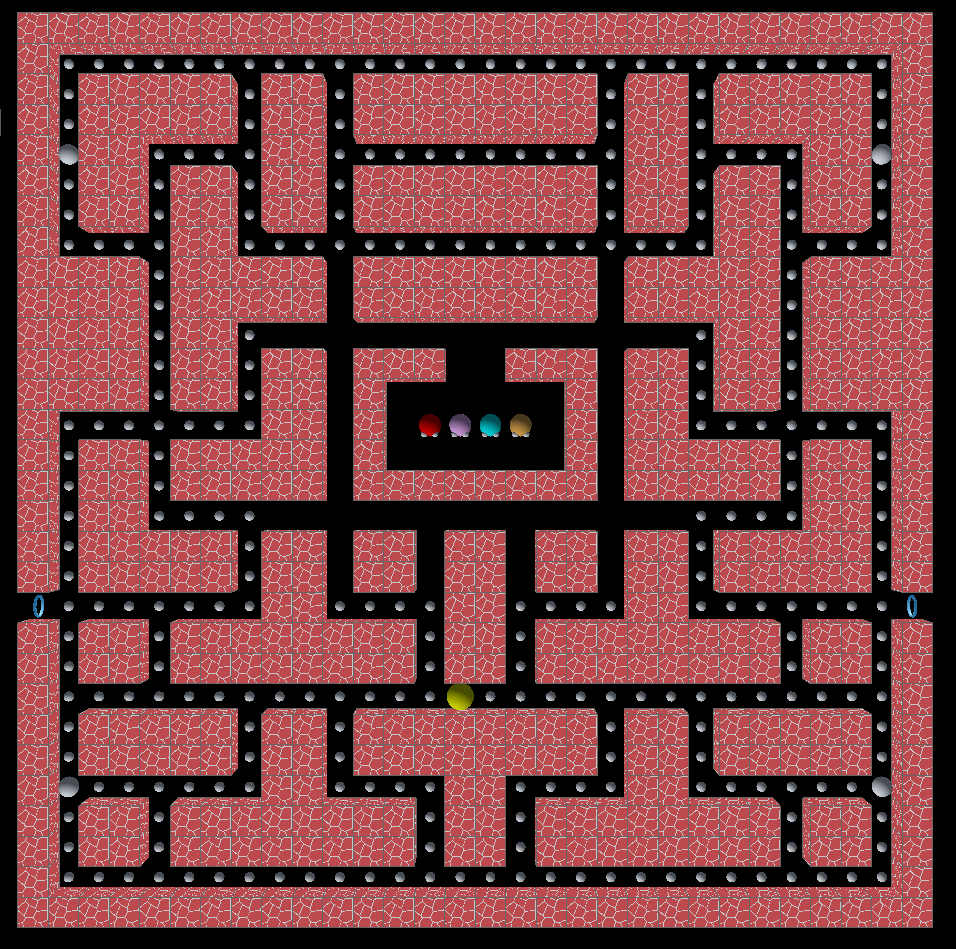
\includegraphics[scale=0.18]{img/laberinto1.png}
        \end{subfigure}
        \hfill
        \begin{subfigure}[b]{0.48\textwidth}
            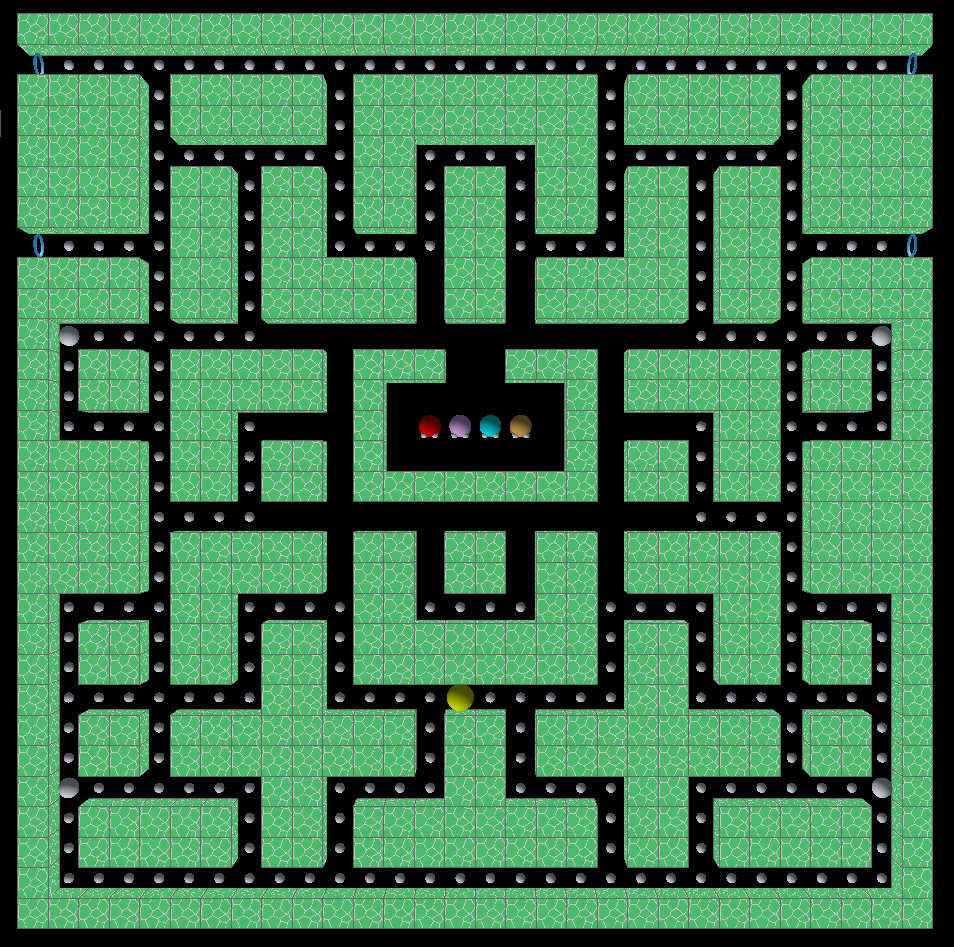
\includegraphics[scale=0.18]{img/laberinto2.png}
        \end{subfigure}
        \vspace{0.2cm}
        \\
        \begin{subfigure}[b]{0.48\textwidth}
            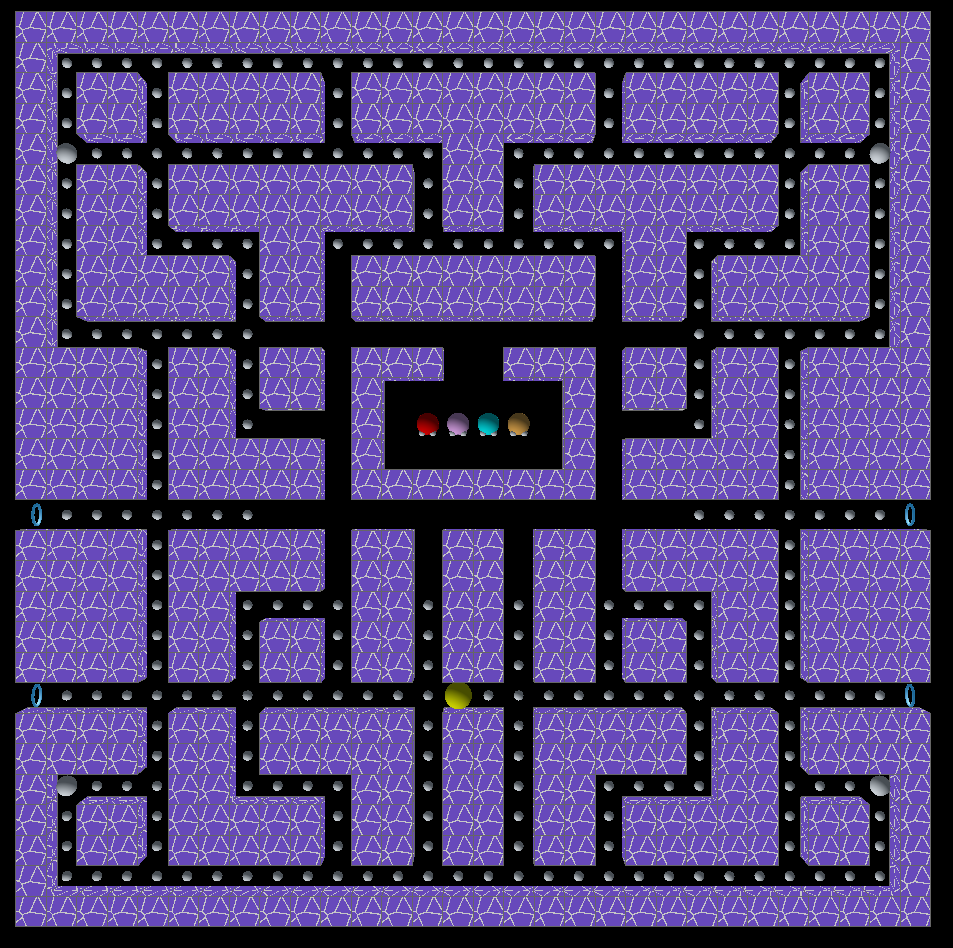
\includegraphics[scale=0.18]{img/laberinto3.png}
        \end{subfigure}
        \hfill
        \begin{subfigure}[b]{0.48\textwidth}
            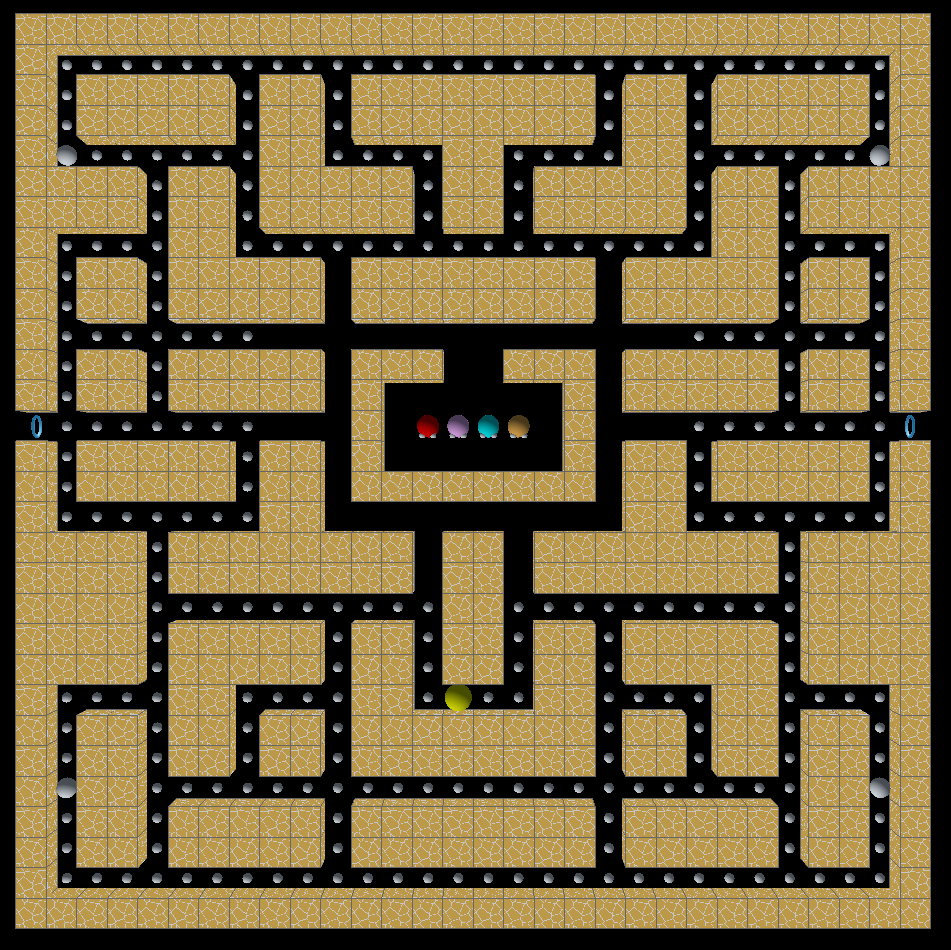
\includegraphics[scale=0.18]{img/laberinto4.png}
        \end{subfigure}
        \vspace{0.2cm}
        \\
        \begin{subfigure}[b]{0.48\textwidth}
            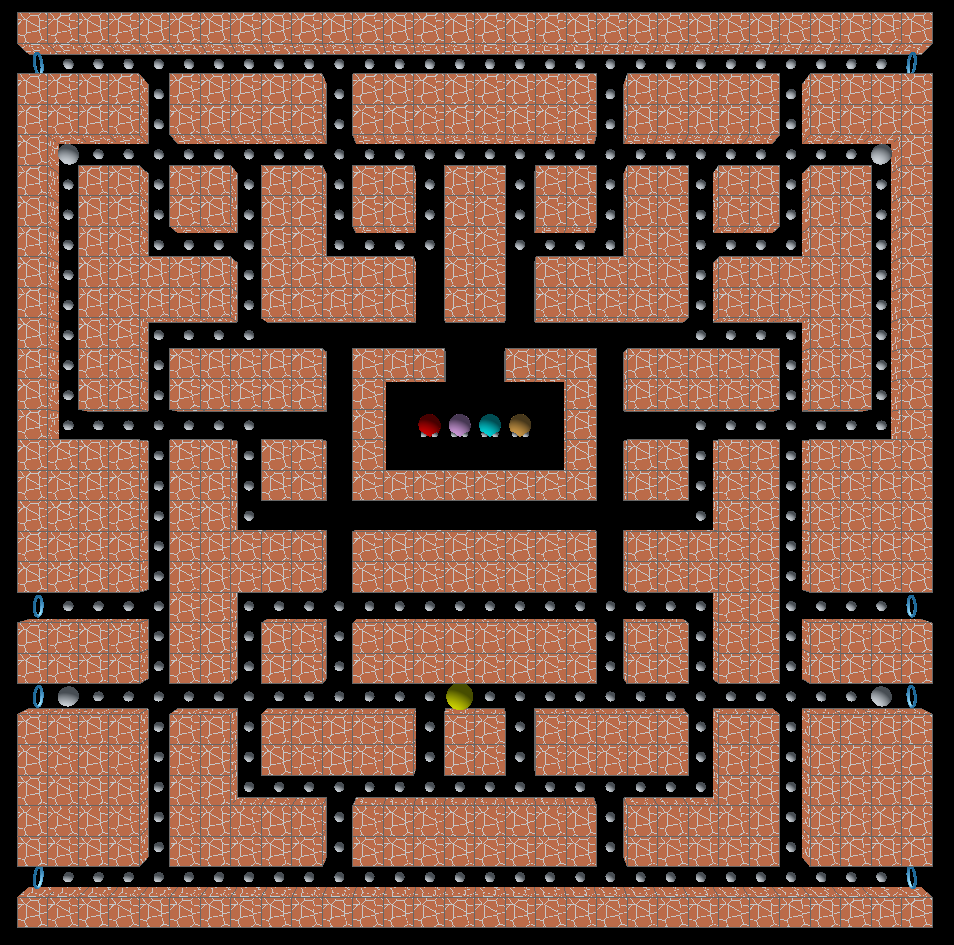
\includegraphics[scale=0.18]{img/laberinto5.png}
        \end{subfigure}
        \hfill
        \begin{subfigure}[b]{0.48\textwidth}
            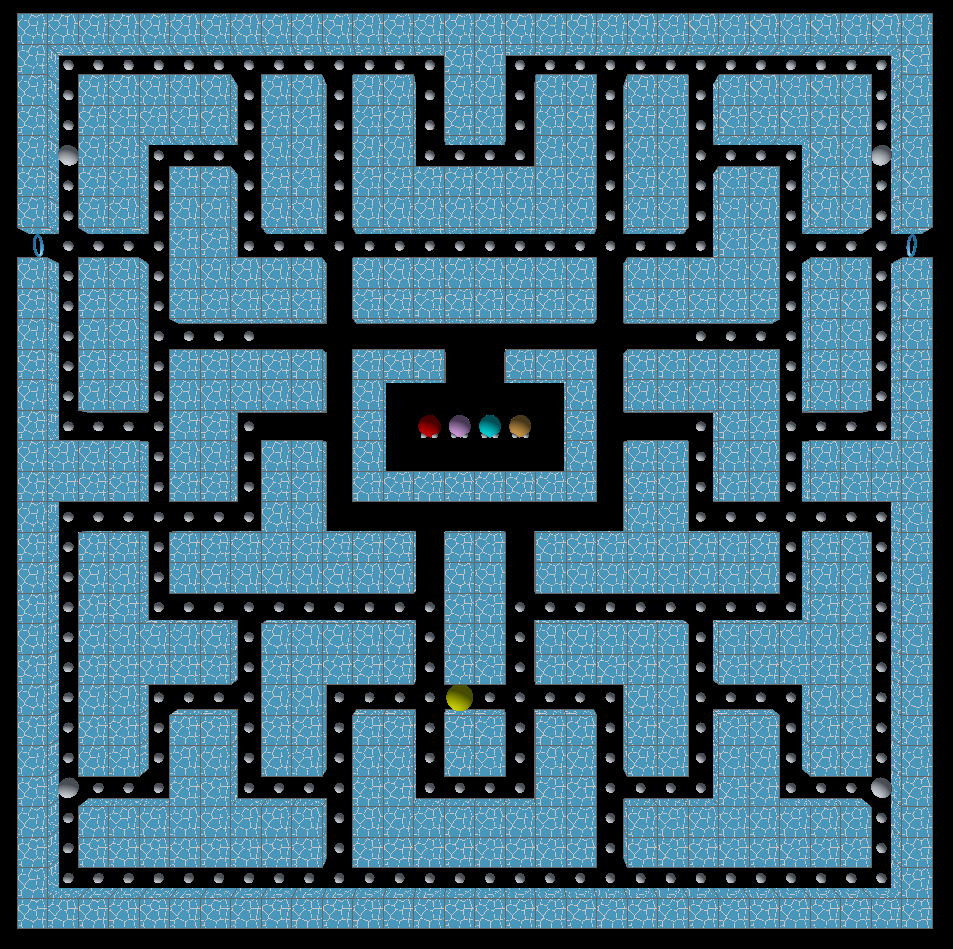
\includegraphics[scale=0.18]{img/laberinto6.png}
        \end{subfigure}
        \caption{Niveles generados procedimentalmente en la reimplementación de Pac-Man.}
        \label{fig:ejemplos}
    \end{figure}

\paragraph{Ejemplo ilustrado del algoritmo de generación de laberintos}\label{par:ejemplo}

A continuación mostramos un ejemplo paso a paso de la ejecución del algoritmo para un caso reducido de dimensión inicial de 4x4.

    \begin{figure}[H]
    \centering
        \begin{subfigure}[b]{0.9\textwidth}
            \centering
            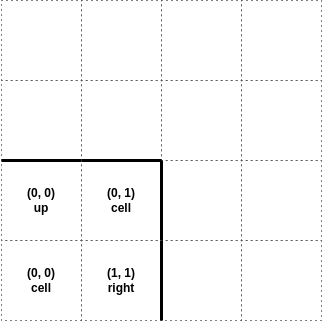
\includegraphics[scale=0.4]{img/paso1.png}
            \caption{Establecemos los valores de las casillas de la casa de los fantasmas.}
        \end{subfigure}
        \par\bigskip
        \begin{subfigure}[b]{0.9\textwidth}
            \centering
            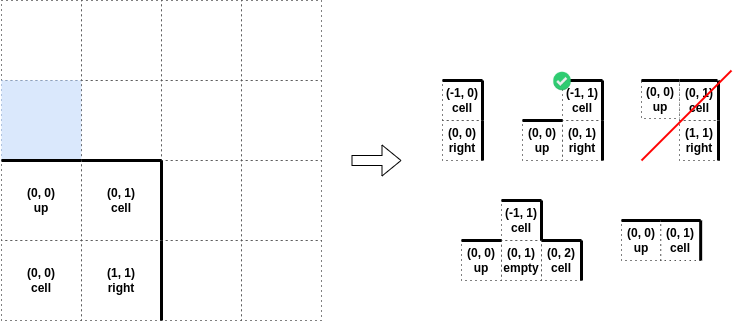
\includegraphics[scale=0.4]{img/paso2.png}
            \caption{Escogemos una casilla de la primera columna, seleccionamos una pieza de entre el conjunto de piezas válidas y la colocamos en nuestra matriz.}
        \end{subfigure}
        \par\bigskip
        \begin{subfigure}[b]{0.9\textwidth}
            \centering
            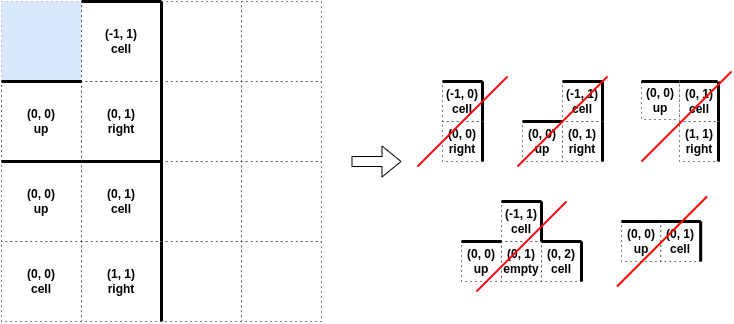
\includegraphics[scale=0.4]{img/paso3.png}
            \caption{Escogemos la única casilla restante de la primera columna. Al ir a seleccionar una pieza y estar vacío el conjunto de piezas válidas, rellenamos la casilla por defecto con una celda completa.}
        \end{subfigure}
        \caption{Ejemplo ilustrado del algoritmo de generación de laberintos - Modelo simple.}
        \label{fig:simple1}
    \end{figure}
    
    \begin{figure}[H]
    \ContinuedFloat 
    \centering
        \begin{subfigure}[b]{0.95\textwidth}
            \centering
            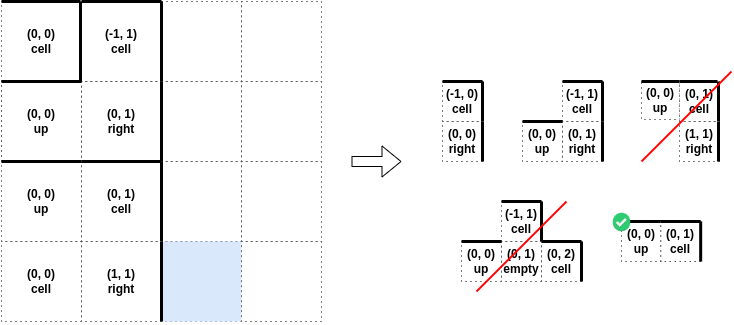
\includegraphics[scale=0.45]{img/paso4.png}
            \caption{Cambiamos a la tercera columna ya que la segunda ya está completa. Escogemos una casilla de la columna, seleccionamos una pieza entre las piezas válidas y la colocamos en nuestra matriz.}
        \end{subfigure}
        \par\bigskip
        \begin{subfigure}[b]{0.95\textwidth}
            \centering
            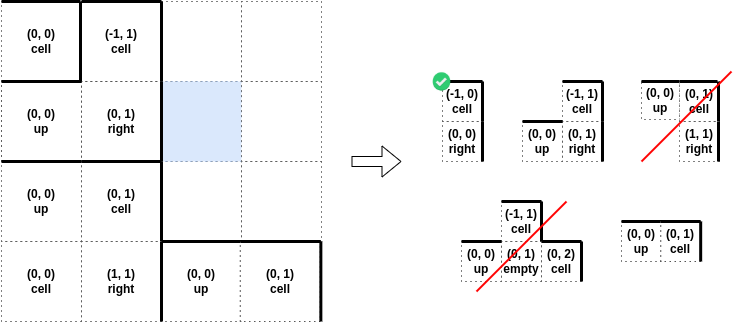
\includegraphics[scale=0.45]{img/paso5.png}
            \caption{Volvemos a repetir el paso anterior. Escogemos una casilla de la columna, seleccionamos una pieza entre las piezas válidas y la colocamos en nuestra matriz.}
        \end{subfigure}
        \par\bigskip
        \begin{subfigure}[b]{0.95\textwidth}
            \centering
            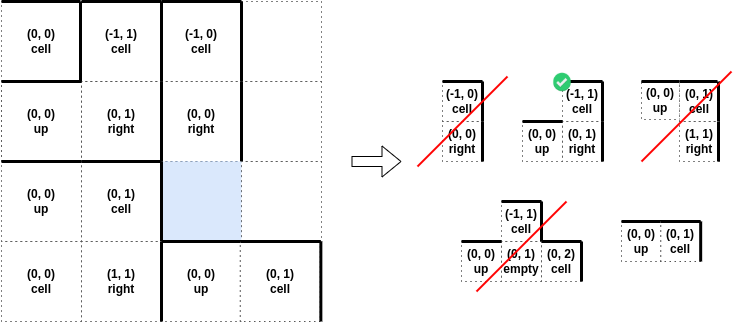
\includegraphics[scale=0.45]{img/paso6.png}
            \caption{Escogemos la única casilla restante de la tercera columnas. Seleccionamos una pieza entre las piezas válidas y la colocamos en nuestra matriz.}
        \end{subfigure}
        \caption{Ejemplo ilustrado del algoritmo de generación de laberintos - Modelo simple.}
        \label{fig:simple2}
    \end{figure}
    
    \begin{figure}[H]
    \ContinuedFloat 
    \centering
        \begin{subfigure}[b]{0.95\textwidth}
            \centering
            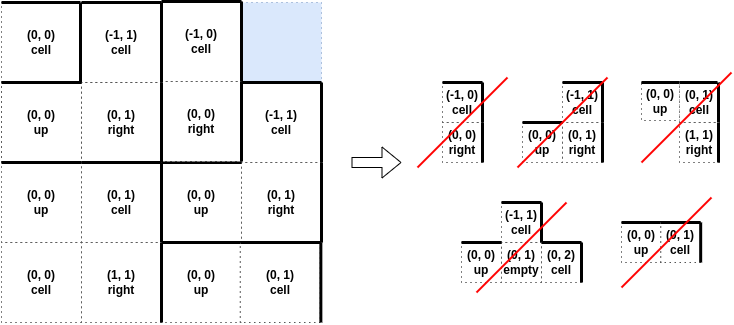
\includegraphics[scale=0.45]{img/paso7.png}
            \caption{Cambiamos a la cuarta columna y escogemos la única casilla restante. Al estar vacío el conjunto de piezas válidas, rellenamos la casilla por defecto con una celda completa.}
        \end{subfigure}
        \par\bigskip
        \begin{subfigure}[b]{0.95\textwidth}
            \centering
            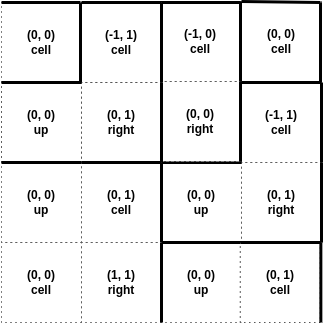
\includegraphics[scale=0.45]{img/paso8.png}
            \caption{Hemos terminado de rellenar la matriz 4x4 que forma el modelo simple.}
        \end{subfigure}
        \par\bigskip
        \begin{subfigure}[b]{0.95\textwidth}
            \centering
            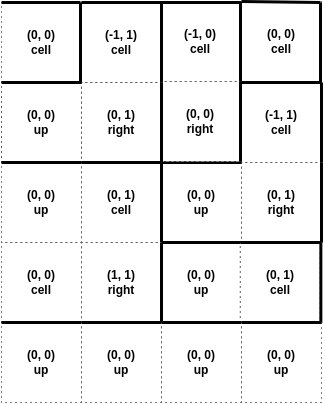
\includegraphics[scale=0.45]{img/paso9.png}
            \caption{Antes de avanzar al modelo de caminos, añadiremos una fila de celdas con borde superior en la parte inferior de nuestra matriz.}
        \end{subfigure}
        \caption{Ejemplo ilustrado del algoritmo de generación de laberintos - Modelo simple.}
        \label{fig:simple3}
    \end{figure}
% ---------------------------------------------------------------------------- %

    \begin{figure}[H]
    \centering
        \begin{subfigure}[b]{0.95\textwidth}
            \centering
            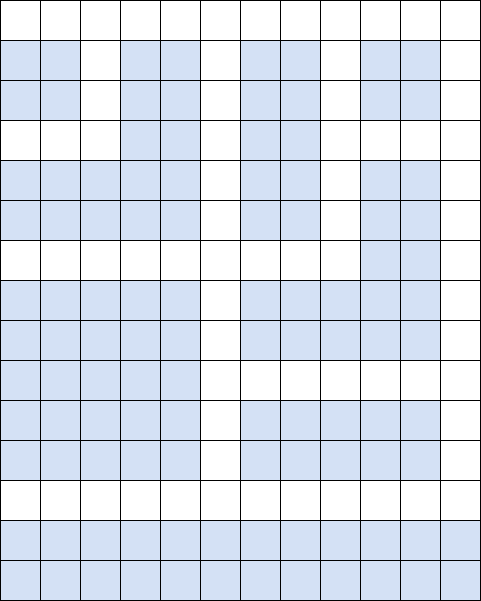
\includegraphics[scale=0.375]{img/paso10.png}
            \caption{Transformamos el modelo simple aplicando las equivalencias de celdas simples a casillas 3x3, dando como resultado una nueva matriz de tamaño 15x12.}
        \end{subfigure}
        \par\bigskip
        \begin{subfigure}[b]{0.45\textwidth}
            \centering
            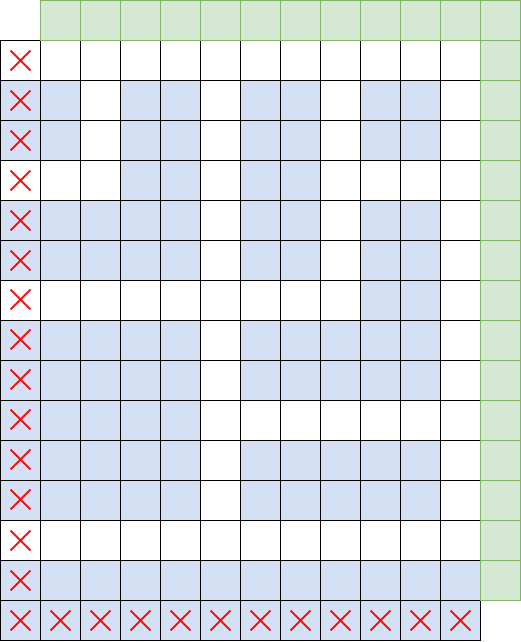
\includegraphics[scale=0.375]{img/paso11.png}
            \caption{Eliminamos la primera columna y la última fila de la matriz resultante. Además, añadimos una fila al principio y una columna al final compuestas exclusivamente de muro.}
        \end{subfigure}
        \hfill\begin{subfigure}[b]{0.45\textwidth}
            \centering
            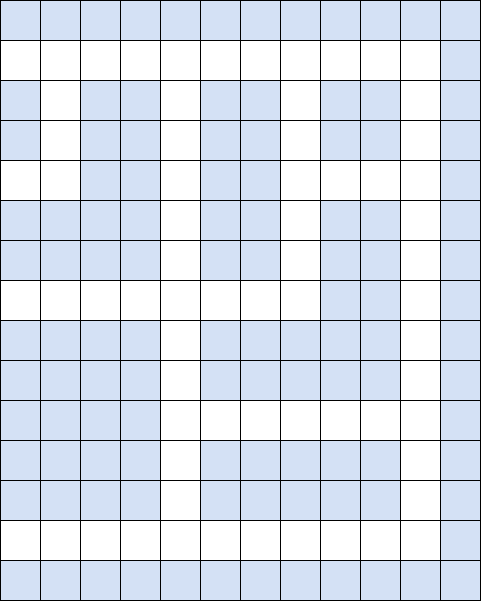
\includegraphics[scale=0.375]{img/paso12.png}
            \caption{Con estas transformaciones y modificaciones hemos completado el modelo de caminos, obteniendo una matriz de tamaño 15x12 compuesta por caminos y muros.}
        \end{subfigure}
        \caption{Ejemplo ilustrado del algoritmo de generación de laberintos - Modelo de caminos.}
        \label{fig:caminos}
    \end{figure}
% ---------------------------------------------------------------------------- %

    \begin{figure}[H]
    \centering
    \begin{subfigure}[b]{0.95\textwidth}
            \centering
            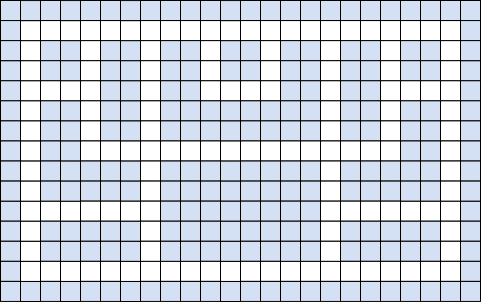
\includegraphics[scale=0.45]{img/paso13.png}
            \caption{Realizamos la simetría respecto al eje Y hacia la izquierda, obteniendo una matriz de 30x15 que forma un laberinto cerrado y válido.}
        \end{subfigure}
        \par\bigskip
        \begin{subfigure}[b]{0.95\textwidth}
            \centering
            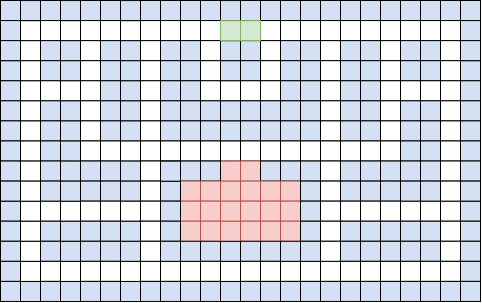
\includegraphics[scale=0.45]{img/paso14.png}
            \caption{Realizamos modificaciones para añadir o quitar muros, como por ejemplo, eliminamos los muros de la zona de la casa de los fantasmas.}
        \end{subfigure}
        
        \par\bigskip
        \begin{subfigure}[b]{0.95\textwidth}
            \centering
            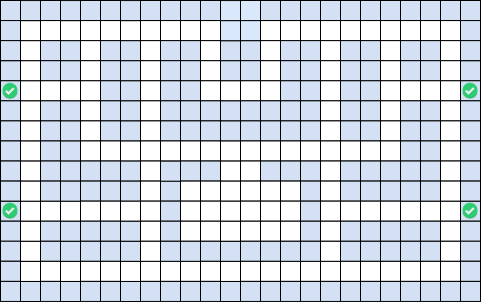
\includegraphics[scale=0.45]{img/paso15.png}
            \caption{En el caso de que no se hayan generado callejones sin salida, seleccionamos los posibles candidatos para la generación de portales, asegurando así que habrá al menos un portal.}
        \end{subfigure}
        \caption{Ejemplo ilustrado del algoritmo de generación de laberintos - Modelo final.}
        \label{fig:final1}
        
    \end{figure}
    
    \begin{figure}[H]
    \ContinuedFloat 
    \centering
    \begin{subfigure}[b]{0.95\textwidth}
            \centering
            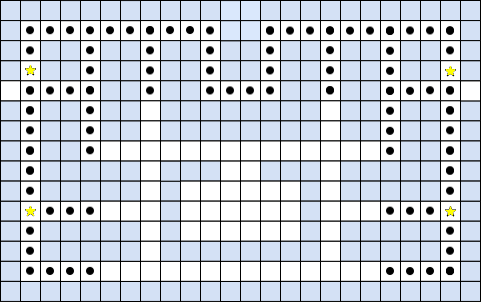
\includegraphics[scale=0.45]{img/paso16.png}
            \caption{Colocamos los puntos dejando una zona libre alrededor de la casa de los fantasmas. Añadimos los potenciadores o pastillas en las cuatro esquinas del mapa.}
        \end{subfigure}
        \par\bigskip
        \begin{subfigure}[b]{0.95\textwidth}
            \centering
            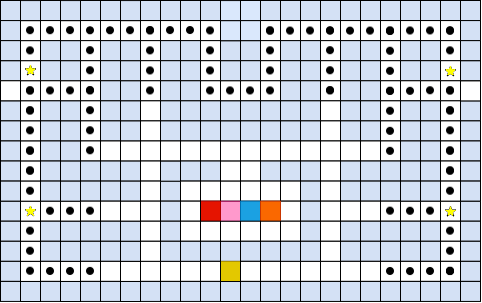
\includegraphics[scale=0.45]{img/paso17.png}
            \caption{Con ello ya dispondríamos de una matriz \textit{MazeData} compuesta por muros, caminos, puntos, pastillas y portales, y que podremos traducir a un nivel generado procedimentalmente del juego \textit{Pac-Man}.}
        \end{subfigure}
        
        \caption{Ejemplo ilustrado del algoritmo de generación de laberintos - Modelo final.}
        \label{fig:final2}
    \end{figure}
% ---------------------------------------------------------------------------- %

\newpage

\subsection{Generación de texturas}

En la implementación se ha trabajado con un shader utilizando el tipo de material \textit{ShaderMaterial} proporcionado por la biblioteca Three.js y partiendo de la implementación de Iñigo Quílez \cite{quilez} de las distancias de Voronoi.\\

Para conseguir lograr variedad de patrones y reducir lo máximo posible las repeticiones o texturas muy similares, hemos jugado con tres factores que afectan a la generación de los patrones de Voronoi. En primer lugar modificamos cada vez que se crea la textura los dos vectores en los que se basa el algoritmo. En segundo lugar variamos la granularidad o cantidad de celdas del patrón, generando patrones con celdas de mayor a menor tamaño. Por último y con el fin de añadir aún más variedad de texturas, modificamos el valor del \textit{Hue} o tonalidad del color.

\begin{table}[H]
    \centering
    \caption{Variables y rango de valores que modifican la textura.}
    \begin{tabular}{|l|l|l|}
    \hline
    Variable & Rango de valores                                                         & Consecuencia                     \\ \hline
    vecA     & \begin{tabular}[c]{@{}l@{}}{[}75.0,150.0)\\ {[}200.0,350.0)\end{tabular} & Modifica el patrón               \\ \hline
    vecB     & \begin{tabular}[c]{@{}l@{}}{[}75.0,150.0)\\ {[}200.0,350.0)\end{tabular} & Modifica el patrón               \\ \hline
    amount   & {[}0.25, 0.5)                                                            & Modifica el tamaño de las celdas \\ \hline
    Hue      & {[}0.0, 1.0)                                                             & Modifica el color                \\ \hline
    \end{tabular}
\end{table}

Estas modificaciones se ejecutan cada vez que generamos un laberinto nuevo, aportando aún más variedad de la ya conseguida con la generación de laberintos implementada en la sección anterior.\\

\begin{figure}[H]
    \begin{center}
        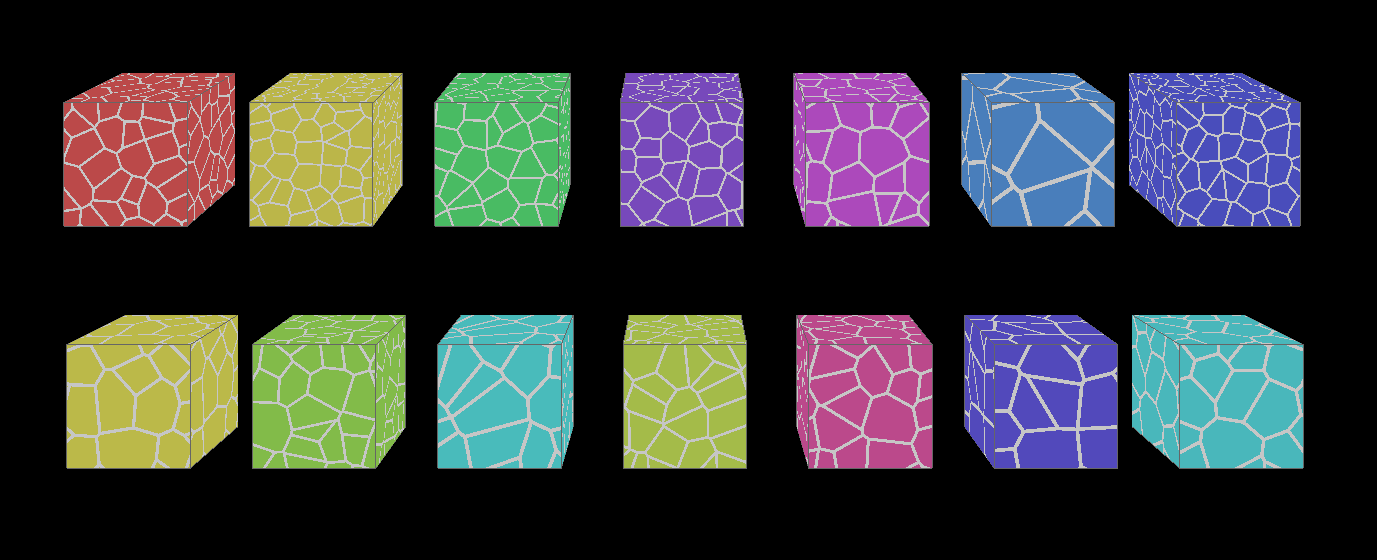
\includegraphics[scale=0.275]{img/texturas.png}
        \caption{Ejemplos de variedad de texturas generadas procedimentalmente usando Teselación de Voronoi.}
    \end{center}
\end{figure}

% ---------------------------------------------------------------------------- %

\newpage

\subsection{Comportamiento de la inteligencia artificial}

Con el fin de generar una dificultad adaptativa a la habilidad del jugador y progresiva según avance la partida, modificaremos tres variables relacionadas con el comportamiento de los fantasmas: tiempo de espera en casa, tiempo que permanecen asustados y que pueden ser comidos por Pac-Man y frecuencia con la que actualizan el camino que están siguiendo.\\

En primer lugar, al reducir el tiempo de espera en casa reducimos la ventana de tiempo en la que el jugador solo tiene que preocuparse por un menor número de enemigos que le persigan.\\

En segundo lugar, al reducir el tiempo que permanecen asustados los fantasmas, reducimos la ventana de tiempo en la que el personaje es invencible y no tiene porqué preocuparse de huir de los enemigos.\\

Por último, al aumentar la frecuencia con la que los fantasmas calculan un nuevo camino hasta la posición de Pac-Man provoca que los fantasmas sean más agresivos y precisos a la hora de localizar al personaje. Podemos ver un resumen de las consecuencias de estas modificaciones del comportamiento y el decremento que se le aplica por nivel a cada variable en la tabla \ref{tab:comportamiento}.\\

\begin{table}[H]
\centering
    \caption{Valores que modifican directa e indirectamente el comportamiento de los fantasmas y generan una dificultad progresiva.}
    
\begin{tabular}{|l|l|l|l|l|}
\hline
Variable                                                         & \begin{tabular}[c]{@{}l@{}}Valor\\ inicial\end{tabular} & \begin{tabular}[c]{@{}l@{}}Decremento\\ por nivel\end{tabular} & \begin{tabular}[c]{@{}l@{}}Valor\\ mínimo\end{tabular} & Efecto                                                                                                                     \\ \hline
\begin{tabular}[c]{@{}l@{}}Tiempo\\ en casa\end{tabular}         & 5s                                                      & 0.1s                                                           & 3s                                                     & \begin{tabular}[c]{@{}l@{}}Menos tiempo sin los cuatro\\ fantasmas en pantalla\end{tabular}                                \\ \hline
\begin{tabular}[c]{@{}l@{}}Tiempo\\ asustado\end{tabular}        & \begin{tabular}[c]{@{}l@{}}10s\\ +5s\end{tabular}       & 0.5s                                                           & \begin{tabular}[c]{@{}l@{}}0.1s\\ +5s\end{tabular}     & \begin{tabular}[c]{@{}l@{}}Menor ventana de tiempo para\\ eliminar a los enemigos\end{tabular}                             \\ \hline
\begin{tabular}[c]{@{}l@{}}Tiempo\\ entre\\ caminos\end{tabular} & 7.5s                                                    & 0.2s                                                           & 2s                                                     & \begin{tabular}[c]{@{}l@{}}Mayor agresividad y precisión\\ de los enemigos a la hora de\\ localizar a Pac-Man\end{tabular} \\ \hline
\end{tabular}
\label{tab:comportamiento}
\end{table}